% Figure: BDG, batch-dispersion guidance. Standalone: pdflatex fig3_bdg.tex
\documentclass[border=4pt]{standalone}
\usepackage{amsmath,amssymb}
\usepackage{tikz}
\usetikzlibrary{arrows.meta,calc,positioning,shapes.geometric}
\definecolor{cB}{HTML}{1F5FA9}
\definecolor{cR}{HTML}{B3261E}
\definecolor{ink}{HTML}{16202C}
\definecolor{mut}{HTML}{5F6A77}
\definecolor{blob}{HTML}{E9F0F8}
\definecolor{band}{HTML}{EAF1FA}
\begin{document}
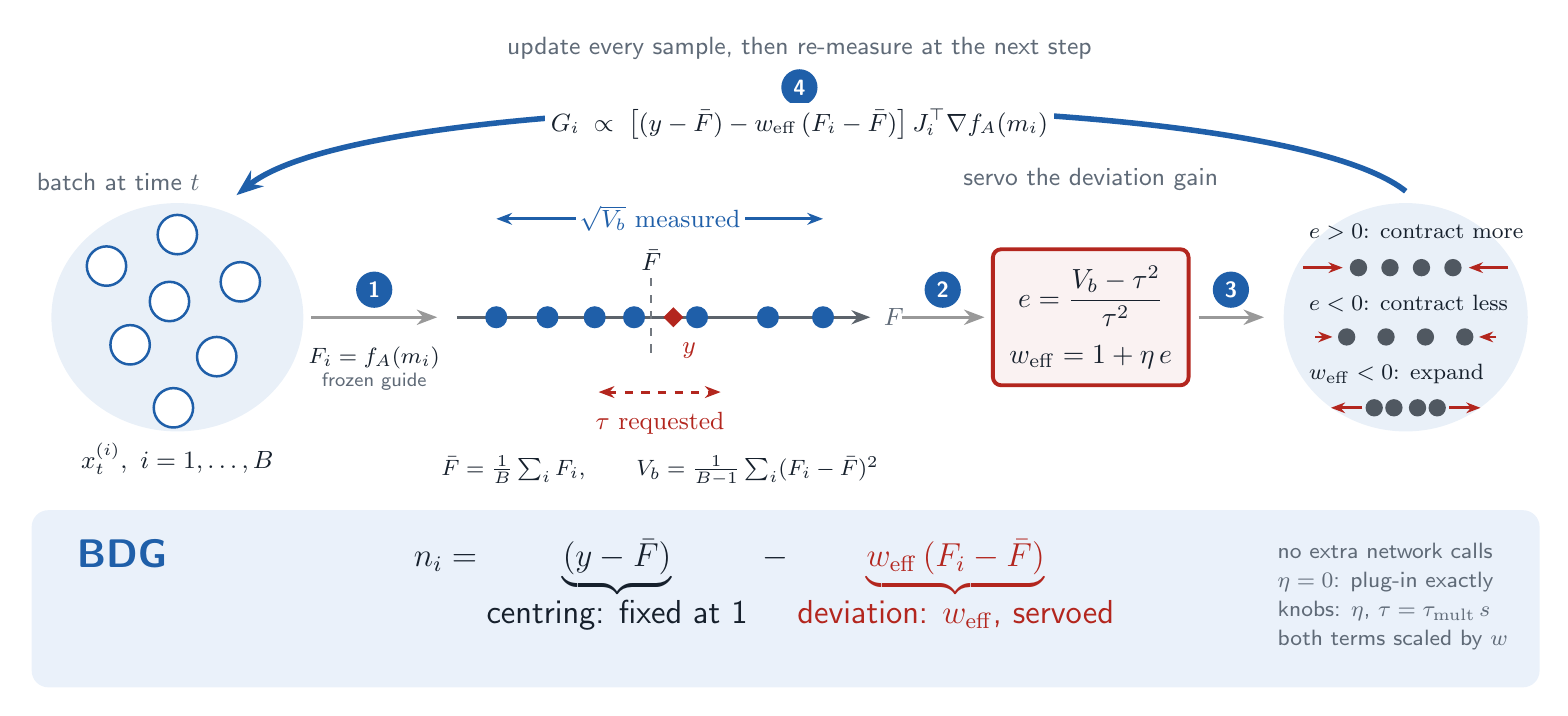
\begin{tikzpicture}[text=ink,
  samp/.style={circle,draw=cB,fill=white,line width=0.9pt,minimum size=5mm,inner sep=0pt},
  fdot/.style={circle,fill=cB,minimum size=2.8mm,inner sep=0pt},
  mdot/.style={circle,fill=ink!75,minimum size=2.2mm,inner sep=0pt},
  ar/.style={-{Stealth[length=2.6mm]},draw=black!40,line width=0.9pt},
  arb/.style={-{Stealth[length=3.4mm]},draw=cB,line width=2pt},
  arr/.style={-{Stealth[length=1.8mm]},draw=cR,line width=1pt},
  num/.style={circle,fill=cB,text=white,font=\sffamily\bfseries\footnotesize,minimum size=4.6mm,inner sep=0pt},
  lab/.style={font=\sffamily\small,text=mut}]

% ---------- (1) the batch at time t ----------
\fill[blob] (1.75,1.7) ellipse (1.6 and 1.45);
\foreach \p in {(0.85,2.35),(1.75,2.75),(2.55,2.15),(1.15,1.35),(2.25,1.2),(1.7,0.55),(1.65,1.9)}
  \node[samp] at \p {};
\node[font=\small] at (1.75,-0.1) {$x_t^{(i)},\ i=1,\dots,B$};
\node[lab] at (1.0,3.42) {batch at time $t$};

% ---------- arrow: score with the frozen guide ----------
\draw[ar] (3.45,1.7) -- (5.05,1.7);
\node[num] at (4.25,2.05) {1};
\node[font=\footnotesize,align=center] at (4.25,1.05) {$F_i=f_A(m_i)$\\[-1pt]{\sffamily\scriptsize\color{mut}frozen guide}};

% ---------- (2) predicted property of the batch ----------
\draw[-{Stealth[length=2.4mm]},line width=0.9pt,draw=ink!70] (5.3,1.7) -- (10.55,1.7);
\node[lab,anchor=west] at (10.6,1.7) {$F$};
\foreach \x in {5.8,6.45,7.05,7.55,8.35,9.25,9.95}
  \node[fdot] at (\x,1.7) {};
\draw[dashed,draw=ink!60,line width=0.8pt] (7.77,1.25) -- (7.77,2.2);
\node[font=\small] at (7.77,2.42) {$\bar F$};
\node[diamond,fill=cR,minimum size=2.6mm,inner sep=0pt] at (8.05,1.7) {};
\node[font=\small,text=cR] at (8.25,1.28) {$y$};
% measured spread (blue) and requested setpoint (red)
\draw[{Stealth[length=2mm]}-{Stealth[length=2mm]},draw=cB,line width=1.1pt] (5.8,2.95) -- (9.95,2.95);
\node[font=\small,text=cB,fill=white,inner sep=1.5pt] at (7.88,2.95) {$\sqrt{V_b}$ measured};
\draw[{Stealth[length=2mm]}-{Stealth[length=2mm]},draw=cR,line width=1.1pt,dashed] (7.1,0.75) -- (8.65,0.75);
\node[font=\small,text=cR,anchor=north] at (7.88,0.62) {$\tau$ requested};
\node[font=\footnotesize] at (7.88,-0.25) {$\bar F=\tfrac1B\sum_i F_i,\qquad V_b=\tfrac{1}{B-1}\sum_i (F_i-\bar F)^2$};

% ---------- arrow: measure ----------
\draw[ar] (10.95,1.7) -- (12.0,1.7);
\node[num] at (11.47,2.05) {2};

% ---------- (3) the controller ----------
\node[draw=cR,line width=1.4pt,fill=cR!6,rounded corners=3pt,inner sep=6pt,align=center] (ctl) at (13.35,1.7)
  {$e=\dfrac{V_b-\tau^2}{\tau^2}$\\[6pt] $w_{\mathrm{eff}}=1+\eta\,e$};
\node[lab] at (13.35,3.45) {servo the deviation gain};

% ---------- arrow: act ----------
\draw[ar] (14.72,1.7) -- (15.55,1.7);
\node[num] at (15.13,2.05) {3};

% ---------- (4) what the gain does ----------
\fill[blob] (17.35,1.7) ellipse (1.55 and 1.45);
% e > 0: contracts more than plug-in
\node[font=\footnotesize,anchor=west] at (16.0,2.78) {$e>0$: contract more};
\foreach \x in {16.75,17.15,17.55,17.95} \node[mdot] at (\x,2.33) {};
\draw[arr] (16.05,2.33) -- (16.55,2.33); \draw[arr] (18.65,2.33) -- (18.15,2.33);
% e < 0 with w_eff > 0: contracts less
\node[font=\footnotesize,anchor=west] at (16.0,1.88) {$e<0$: contract less};
\foreach \x in {16.6,17.1,17.6,18.1} \node[mdot] at (\x,1.45) {};
\draw[arr] (16.2,1.45) -- (16.42,1.45); \draw[arr] (18.5,1.45) -- (18.28,1.45);
% w_eff < 0: expands
\node[font=\footnotesize,anchor=west] at (16.0,0.98) {$w_{\mathrm{eff}}<0$: expand};
\foreach \x in {16.95,17.2,17.5,17.75} \node[mdot] at (\x,0.55) {};
\draw[arr] (16.8,0.55) -- (16.4,0.55); \draw[arr] (17.9,0.55) -- (18.3,0.55);

% ---------- feedback: the next step re-measures ----------
\draw[arb] (17.35,3.3) .. controls (15.6,4.7) and (4.3,4.7) .. (2.5,3.25);
\node[num] at (9.65,4.62) {4};
\node[font=\small,fill=white,inner sep=2pt] at (9.65,4.15) {$G_i\;\propto\;\big[(y-\bar F)-w_{\mathrm{eff}}\,(F_i-\bar F)\big]\,J_i^{\top}\nabla f_A(m_i)$};
\node[lab] at (9.65,5.12) {update every sample, then re-measure at the next step};

% ---------- the rule ----------
\fill[band,rounded corners=6pt] (-0.1,-3.0) rectangle (19.05,-0.75);
\node[font=\sffamily\bfseries\Large,text=cB,anchor=west] at (0.35,-1.3) {BDG};
\node at (9.2,-1.72) {\large$n_i=
  \underbrace{(y-\bar F)}_{\textstyle\text{\sffamily centring: fixed at 1}}
  \;-\;
  \textcolor{cR}{\underbrace{w_{\mathrm{eff}}\,(F_i-\bar F)}_{\textstyle\text{\sffamily deviation: } w_{\mathrm{eff}}\text{\sffamily, servoed}}}$};
\node[font=\sffamily\footnotesize,text=mut,align=left,anchor=west] at (15.6,-1.85)
  {no extra network calls\\[1pt] $\eta=0$: plug-in exactly\\[1pt] knobs: $\eta$, $\tau=\tau_{\mathrm{mult}}\,s$\\[1pt] both terms scaled by $w$};
\end{tikzpicture}
\end{document}
